\section{Data Analysis}

In this section, we present our results after the execution of sorting algorithms over the input files. We analyzed only the dependent variables \textit{percentage of the largest subarray size ((\%LSS)} and \textit{percentage of unordered elements quantity (\%UEQ)}. These variables, because they are a percentage value, already were normalized (i.e., the same order of magnitude) related to dependent variable array size.

\subsection{Exploratory Data Analysis (EDA)}

Firstly, we performed an analysis of the distribution of the dependent variables \%LSS and \%UEQ. To help in this task, we produced histograms, boxplot graphs, tables containing data about mean, median, standard deviation, and the minimum and maximum values.

The following Figures \ref{fig-histogram-boxplot-bubble-001100}, \ref{fig-histogram-boxplot-insertion-001100}, \ref{fig-histogram-boxplot-merge-00510000} and \ref{fig-histogram-boxplot-quick-00510000} illustrates examples of histograms and boxplot graphs for each combination of \textit{Algorithm X Probability of Failure X Array Size}. In each of those figures, the graphs were exhibited over the dependent variables \%LSS and \%UEQ.  In the histogram, the red vertical line means the mean, and the blue vertical line means the median. On the other hand, in the boxplot, the red horizontal line means the mean, and the blue horizontal line means the median.

\begin{figure}[H]
    \centering
    \frame{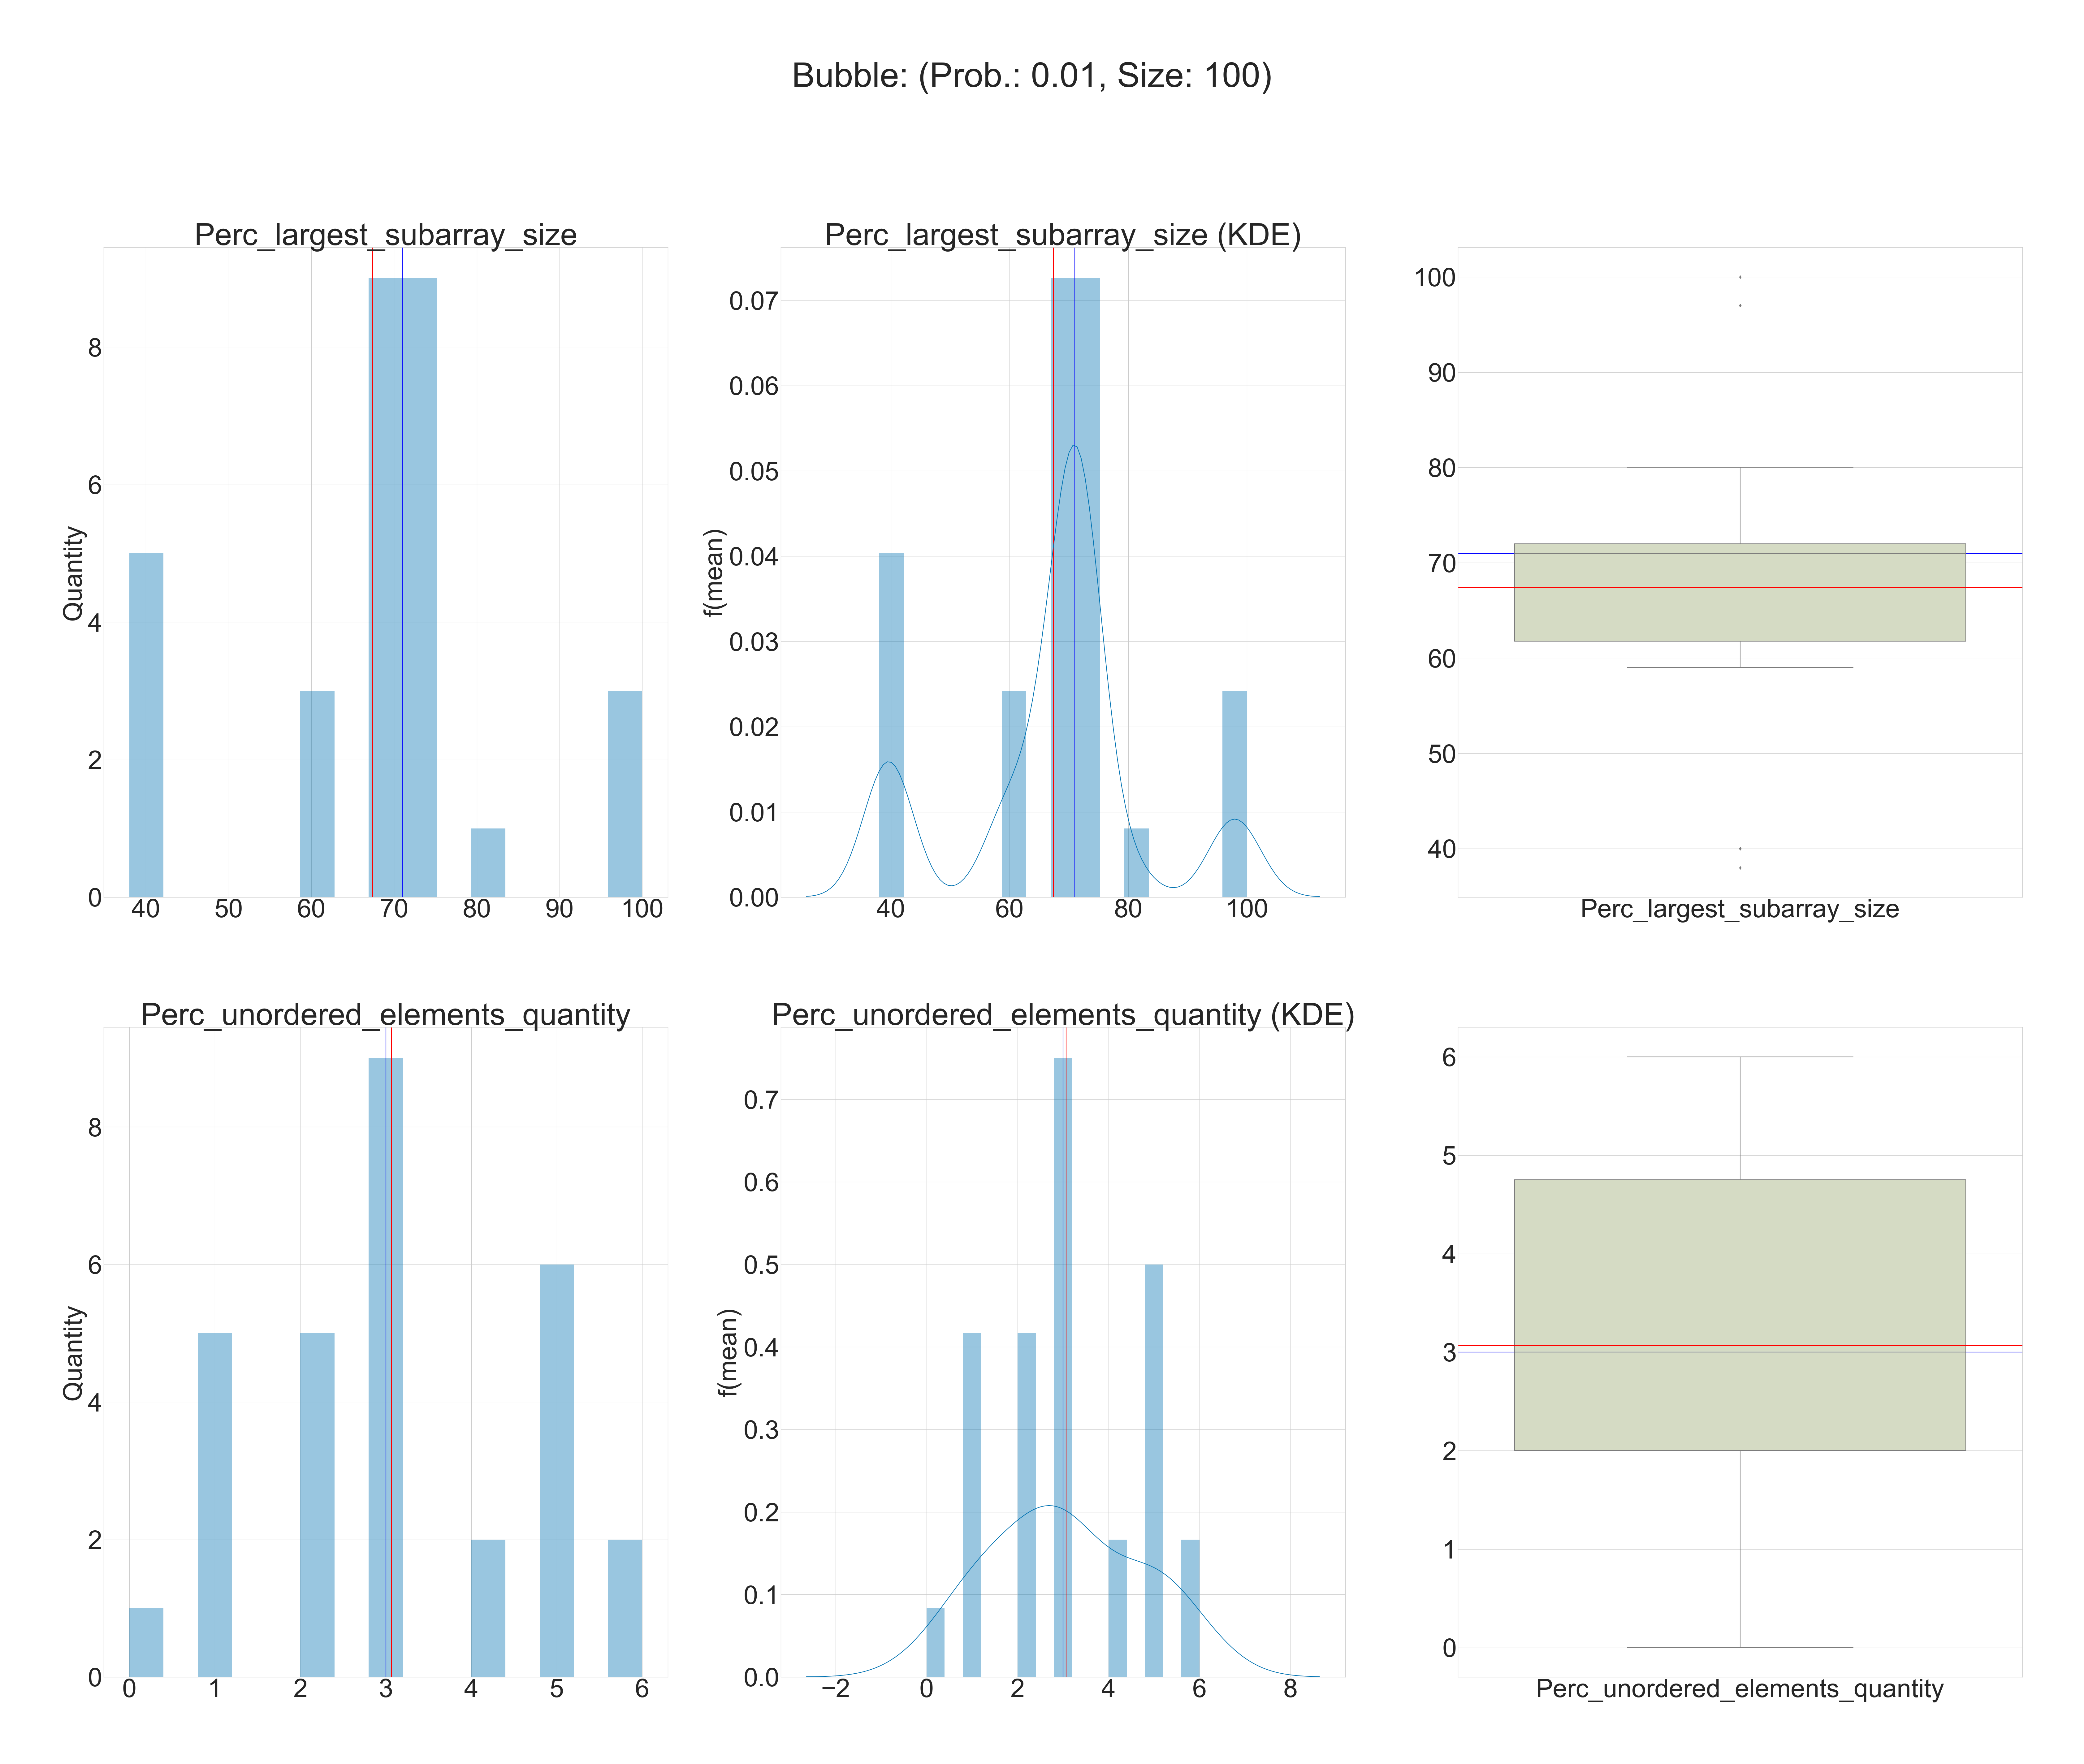
\includegraphics[scale=0.105]{figures/0_01_100_Bubble.png}}
    \caption{Histograms and Boxplot for Bubblesort, with \textit{probability of failure} of 0.01 and \textit{array size} of 100.}
    \label{fig-histogram-boxplot-bubble-001100}
\end{figure}

Based on Figures \ref{fig-histogram-boxplot-bubble-001100}, \ref{fig-histogram-boxplot-insertion-001100}, \ref{fig-histogram-boxplot-merge-00510000} and \ref{fig-histogram-boxplot-quick-00510000}, the following Tables \ref{tab-distribution-depentent-variable-ueq} and \ref{tab-distribution-depentent-variable-lss} illustrates the information about the dependent variables (\%LSS and \%UEQ) distribution.

\begin{table}[H]
    \caption{Table Type Styles}
    \begin{center}
    \begin{tabular}{|c|c|c|c|c|c|c|c|}
    \hline
    \textbf{Prob. of Failure} & \textbf{Array Size} & \textbf{Algorithm} & \multicolumn{5}{|c|}{\textbf{Percentage of unordered elements quantity (\%UEQ)}} \\
    \cline{4-8} 
    & & & \textbf{\textit{Mean}}& \textbf{\textit{Median}} & \textbf{\textit{Std. Deviation}} & \textbf{\textit{Minimum}} & \textbf{\textit{Maximum}} \\
    \hline
    0.01 & 100 & bubble & 3.07 & 3.0 & 1.64 & 0.0 & 6.0 \\
    \hline
    0.01 & 100 & insertion & 10.87 & 11.0 & 1.59 & 8.0 & 14.0 \\
    \hline
    0.05 & 10000 & merge & 28.32 & 28.34 & 0.31 & 27.69 & 28.86 \\
    \hline
    0.05 & 10000 & quick & 19.56 & 19.58 & 0.26 & 18.95 & 20.07 \\
    \hline
    \end{tabular}
    \label{tab-distribution-depentent-variable-ueq}
    \end{center}
\end{table}

\begin{figure}[H]
    \centering
    \frame{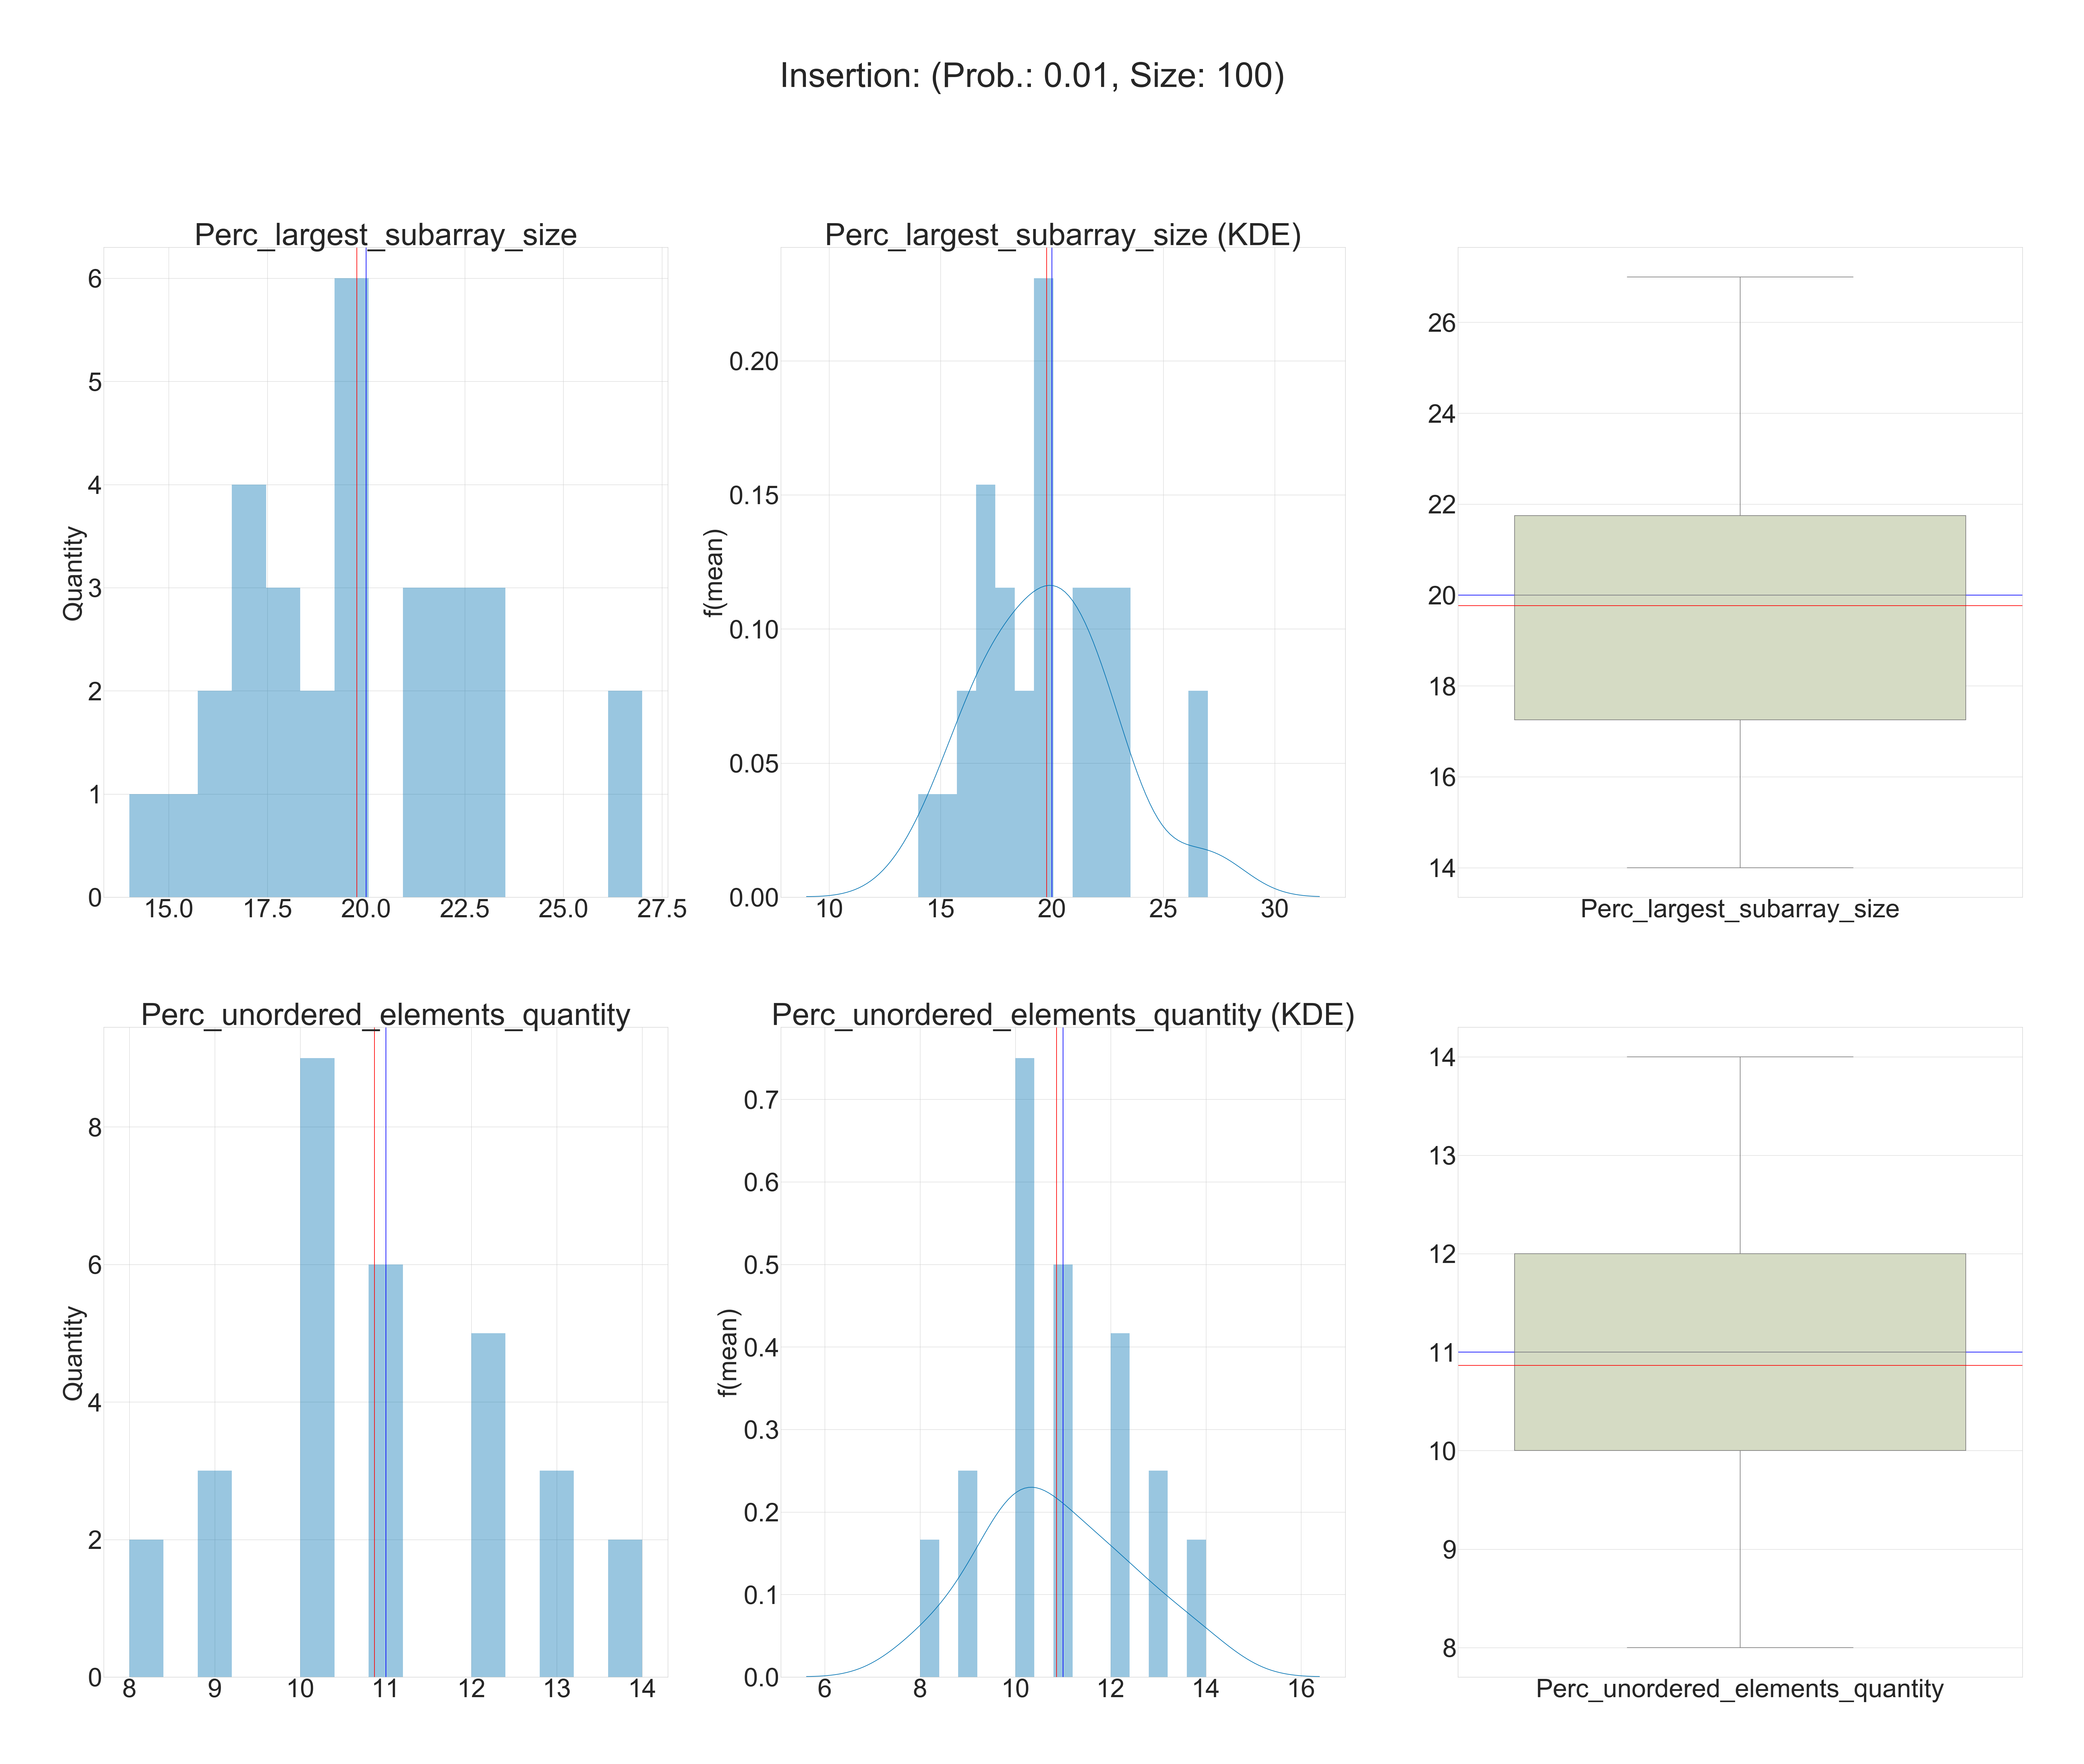
\includegraphics[scale=0.105]{figures/0_01_100_Insertion.png}}
    \caption{Histograms and Boxplot for Insertion sort, with \textit{probability of failure} of 0.01 and \textit{array size} of 100.}
    \label{fig-histogram-boxplot-insertion-001100}
\end{figure}

\begin{table}[H]
    \caption{Table Type Styles}
    \begin{center}
    \begin{tabular}{|c|c|c|c|c|c|c|c|}
    \hline
    \textbf{Prob. of Failure} & \textbf{Array Size} & \textbf{Algorithm} & \multicolumn{5}{|c|}{\textbf{Percentage of largest subarray size (\%LSS)}} \\
    \cline{4-8} 
    & & & \textbf{\textit{Mean}}& \textbf{\textit{Median}} & \textbf{\textit{Std. Deviation}} & \textbf{\textit{Minimum}} & \textbf{\textit{Maximum}} \\
    \hline
    0.01 & 100 & bubble & 67.4 & 71.0 & 15.84 & 38.0 & 100.0 \\
    \hline
    0.01 & 100 & insertion & 19.77 & 20.0 & 3.11 & 14.0 & 27.0 \\
    \hline
    0.05 & 10000 & merge & 0.19 & 0.2 & 0.03 & 0.15 & 28.86 \\
    \hline
    0.05 & 10000 & quick & 0.3 & 0.3 & 0.03 & 0.23 & 0.34 \\
    \hline
    \end{tabular}
    \label{tab-distribution-depentent-variable-lss}
    \end{center}
\end{table}

\begin{figure}[H]
    \centering
    \frame{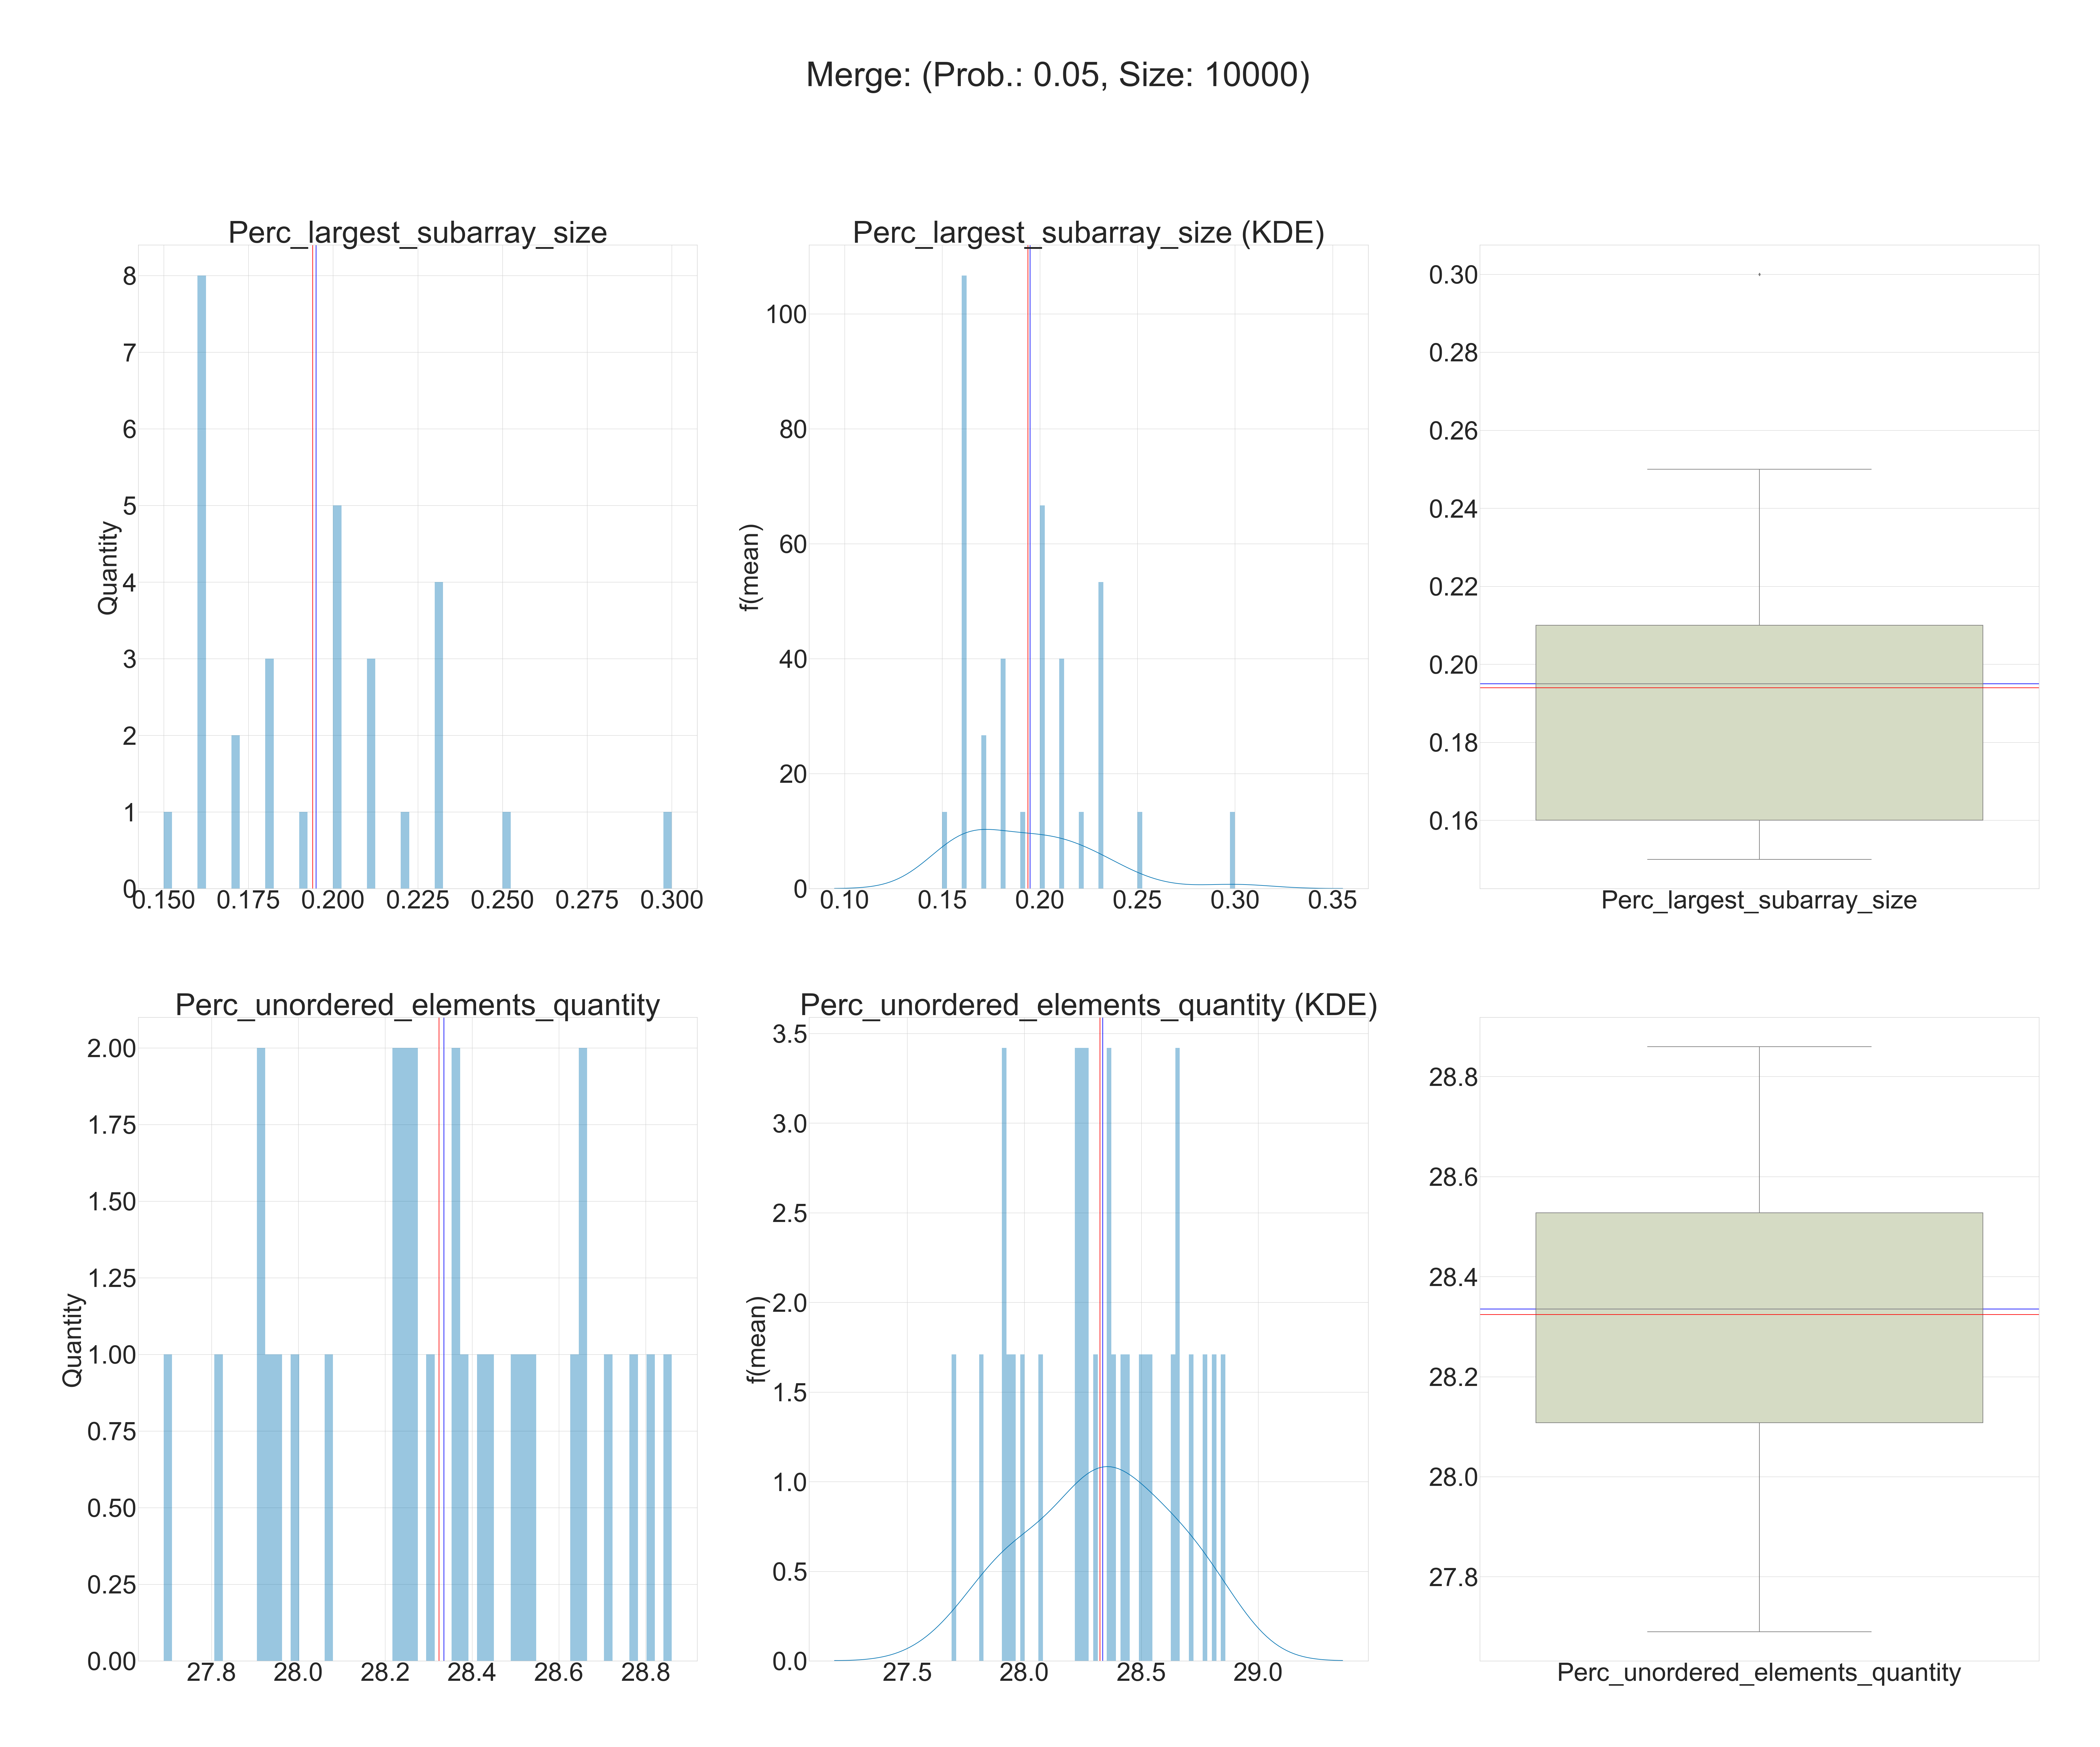
\includegraphics[scale=0.105]{figures/0_05_10000_Merge.png}}
    \caption{Histograms and Boxplot for Mergesort, with \textit{probability of failure} of 0.05 and \textit{array size} of 10000.}
    \label{fig-histogram-boxplot-merge-00510000}
\end{figure}

\begin{figure}[H]
    \centering
    \frame{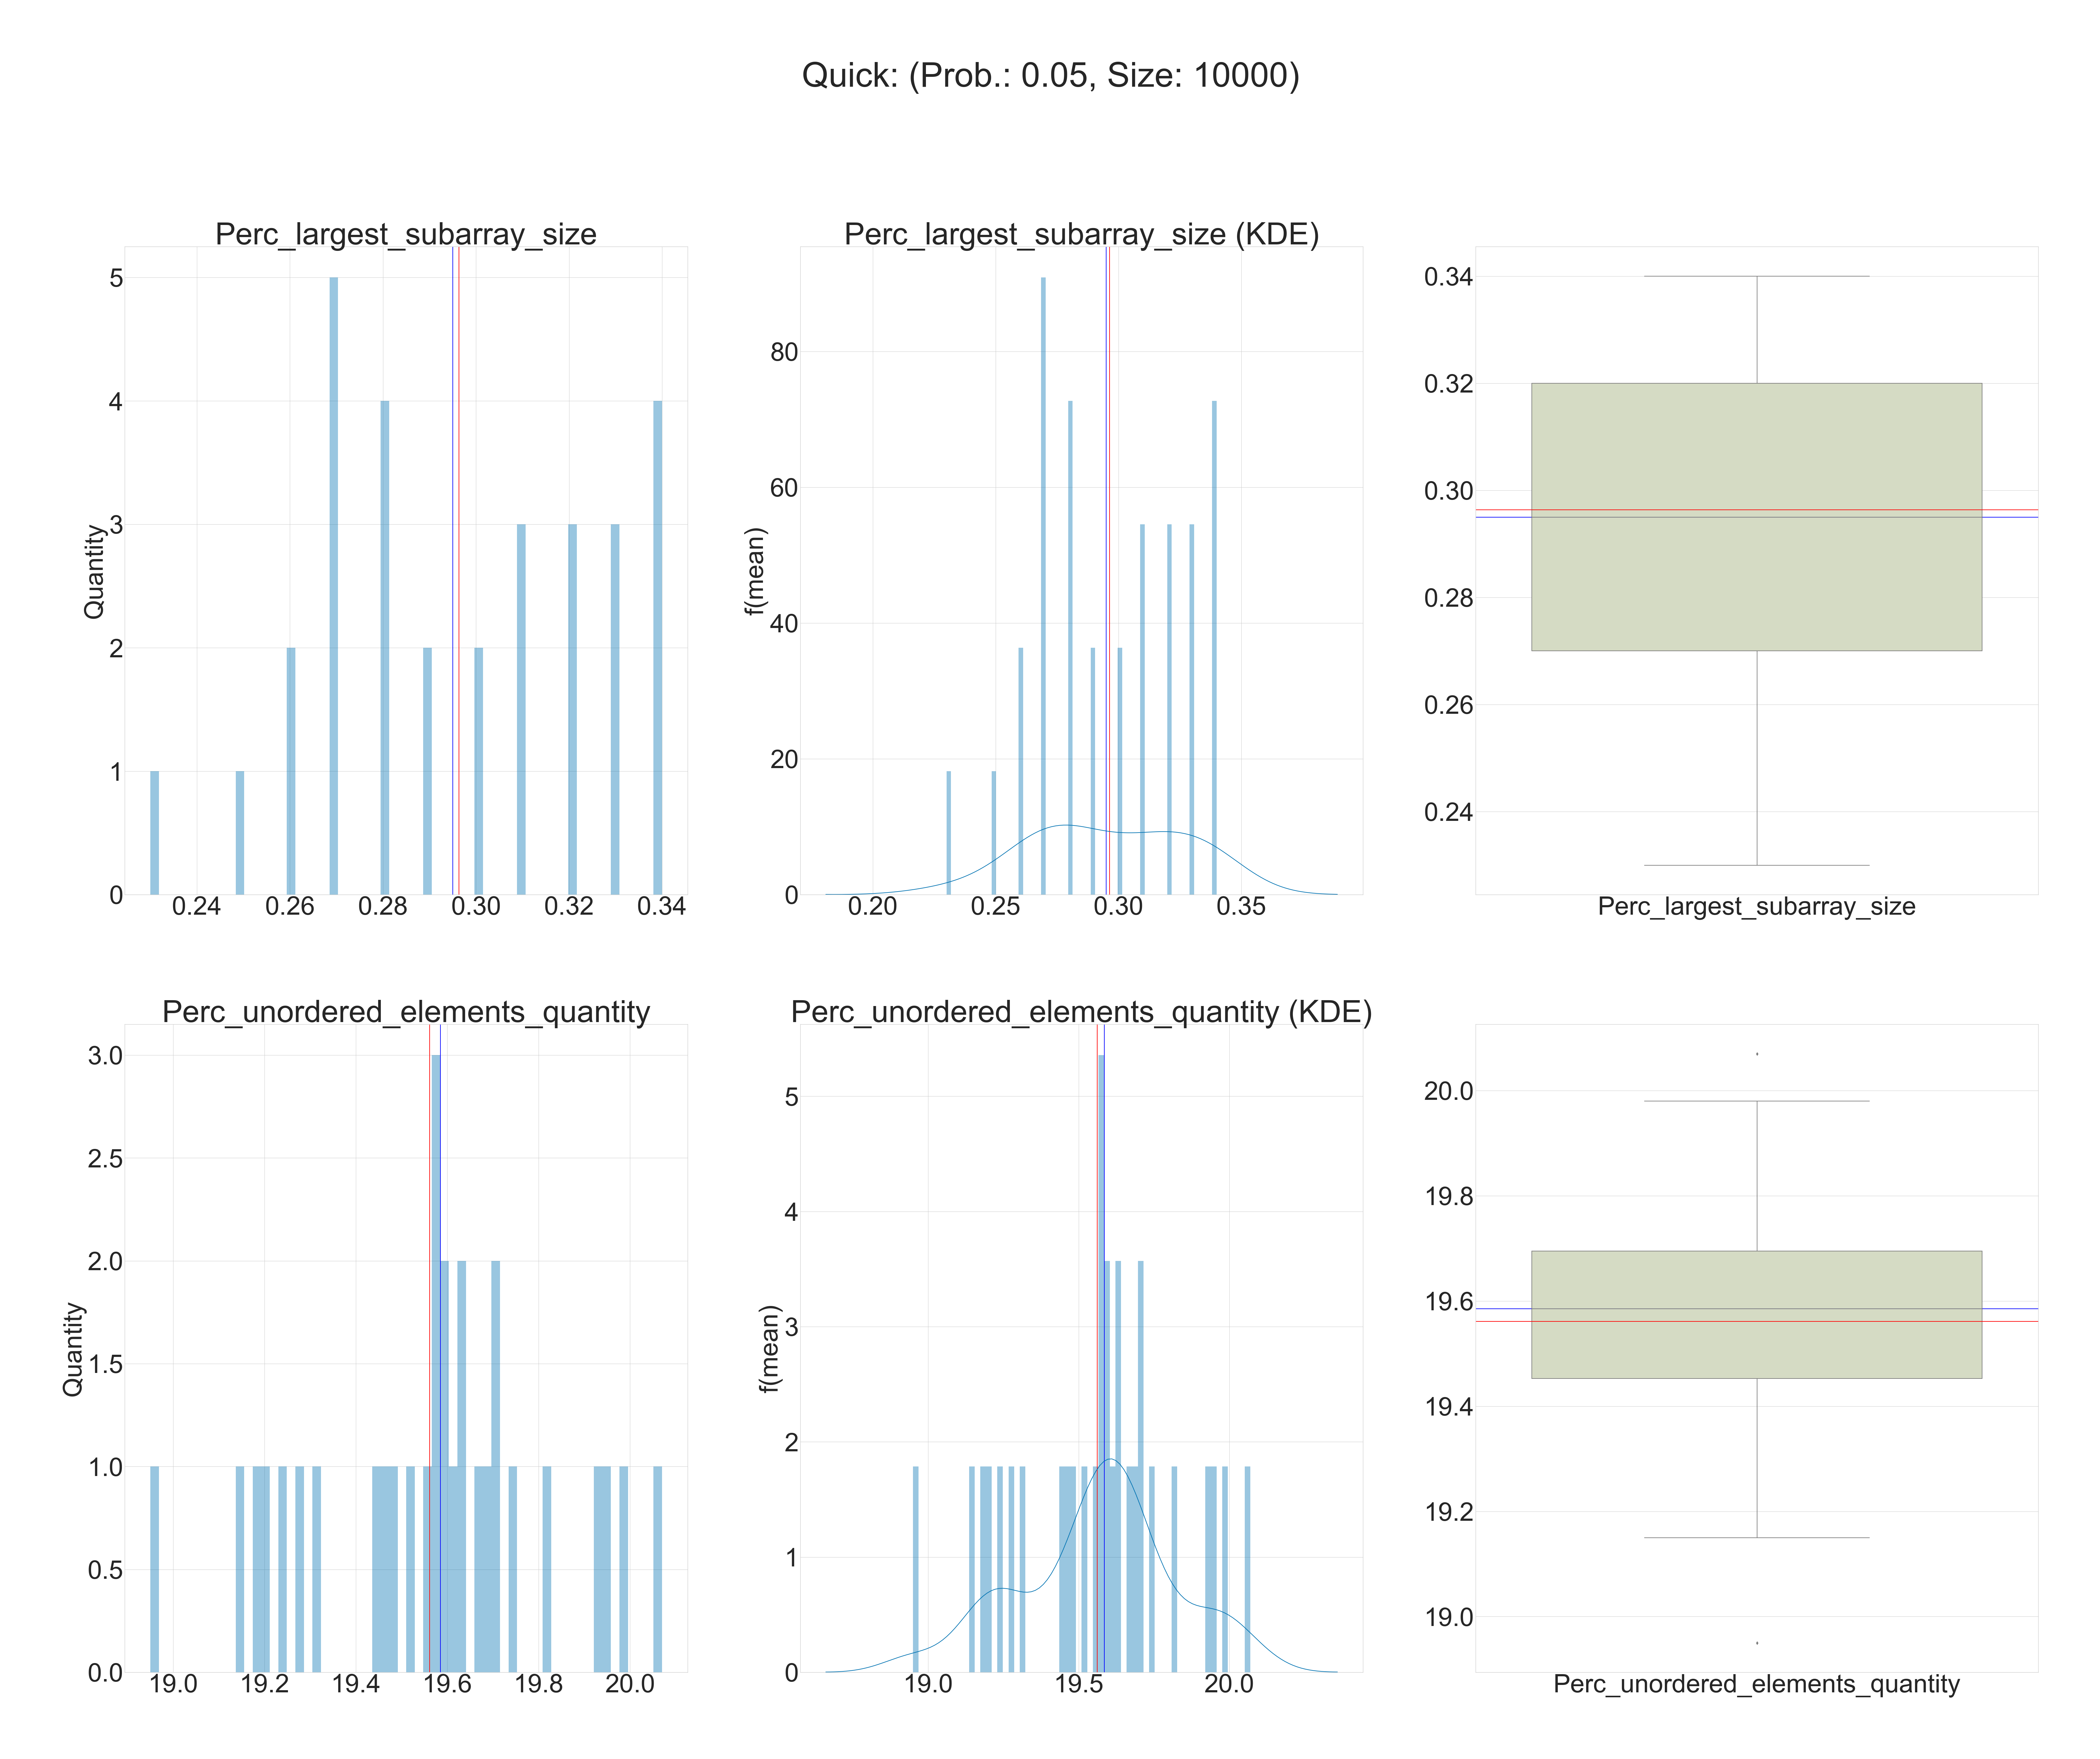
\includegraphics[scale=0.105]{figures/0_05_10000_Quick.png}}
    \caption{Histograms and Boxplot for Quicksort, with \textit{probability of failure} of 0.05 and \textit{array size} of 10000.}
    \label{fig-histogram-boxplot-quick-00510000}
\end{figure}

We produced graphs with the same data showed in Tables \ref{tab-distribution-depentent-variable-ueq} and \ref{tab-distribution-depentent-variable-lss}. Figure \ref{fig-distribution-all-algorithms-001-all-sizes} shows an example of these graphs. On it, we illustrate on the top-left graph that, considering the mean, bubblesort produces fewer unordered elements related to the total than other algorithms.

\begin{figure}[H]
    \centering
    \frame{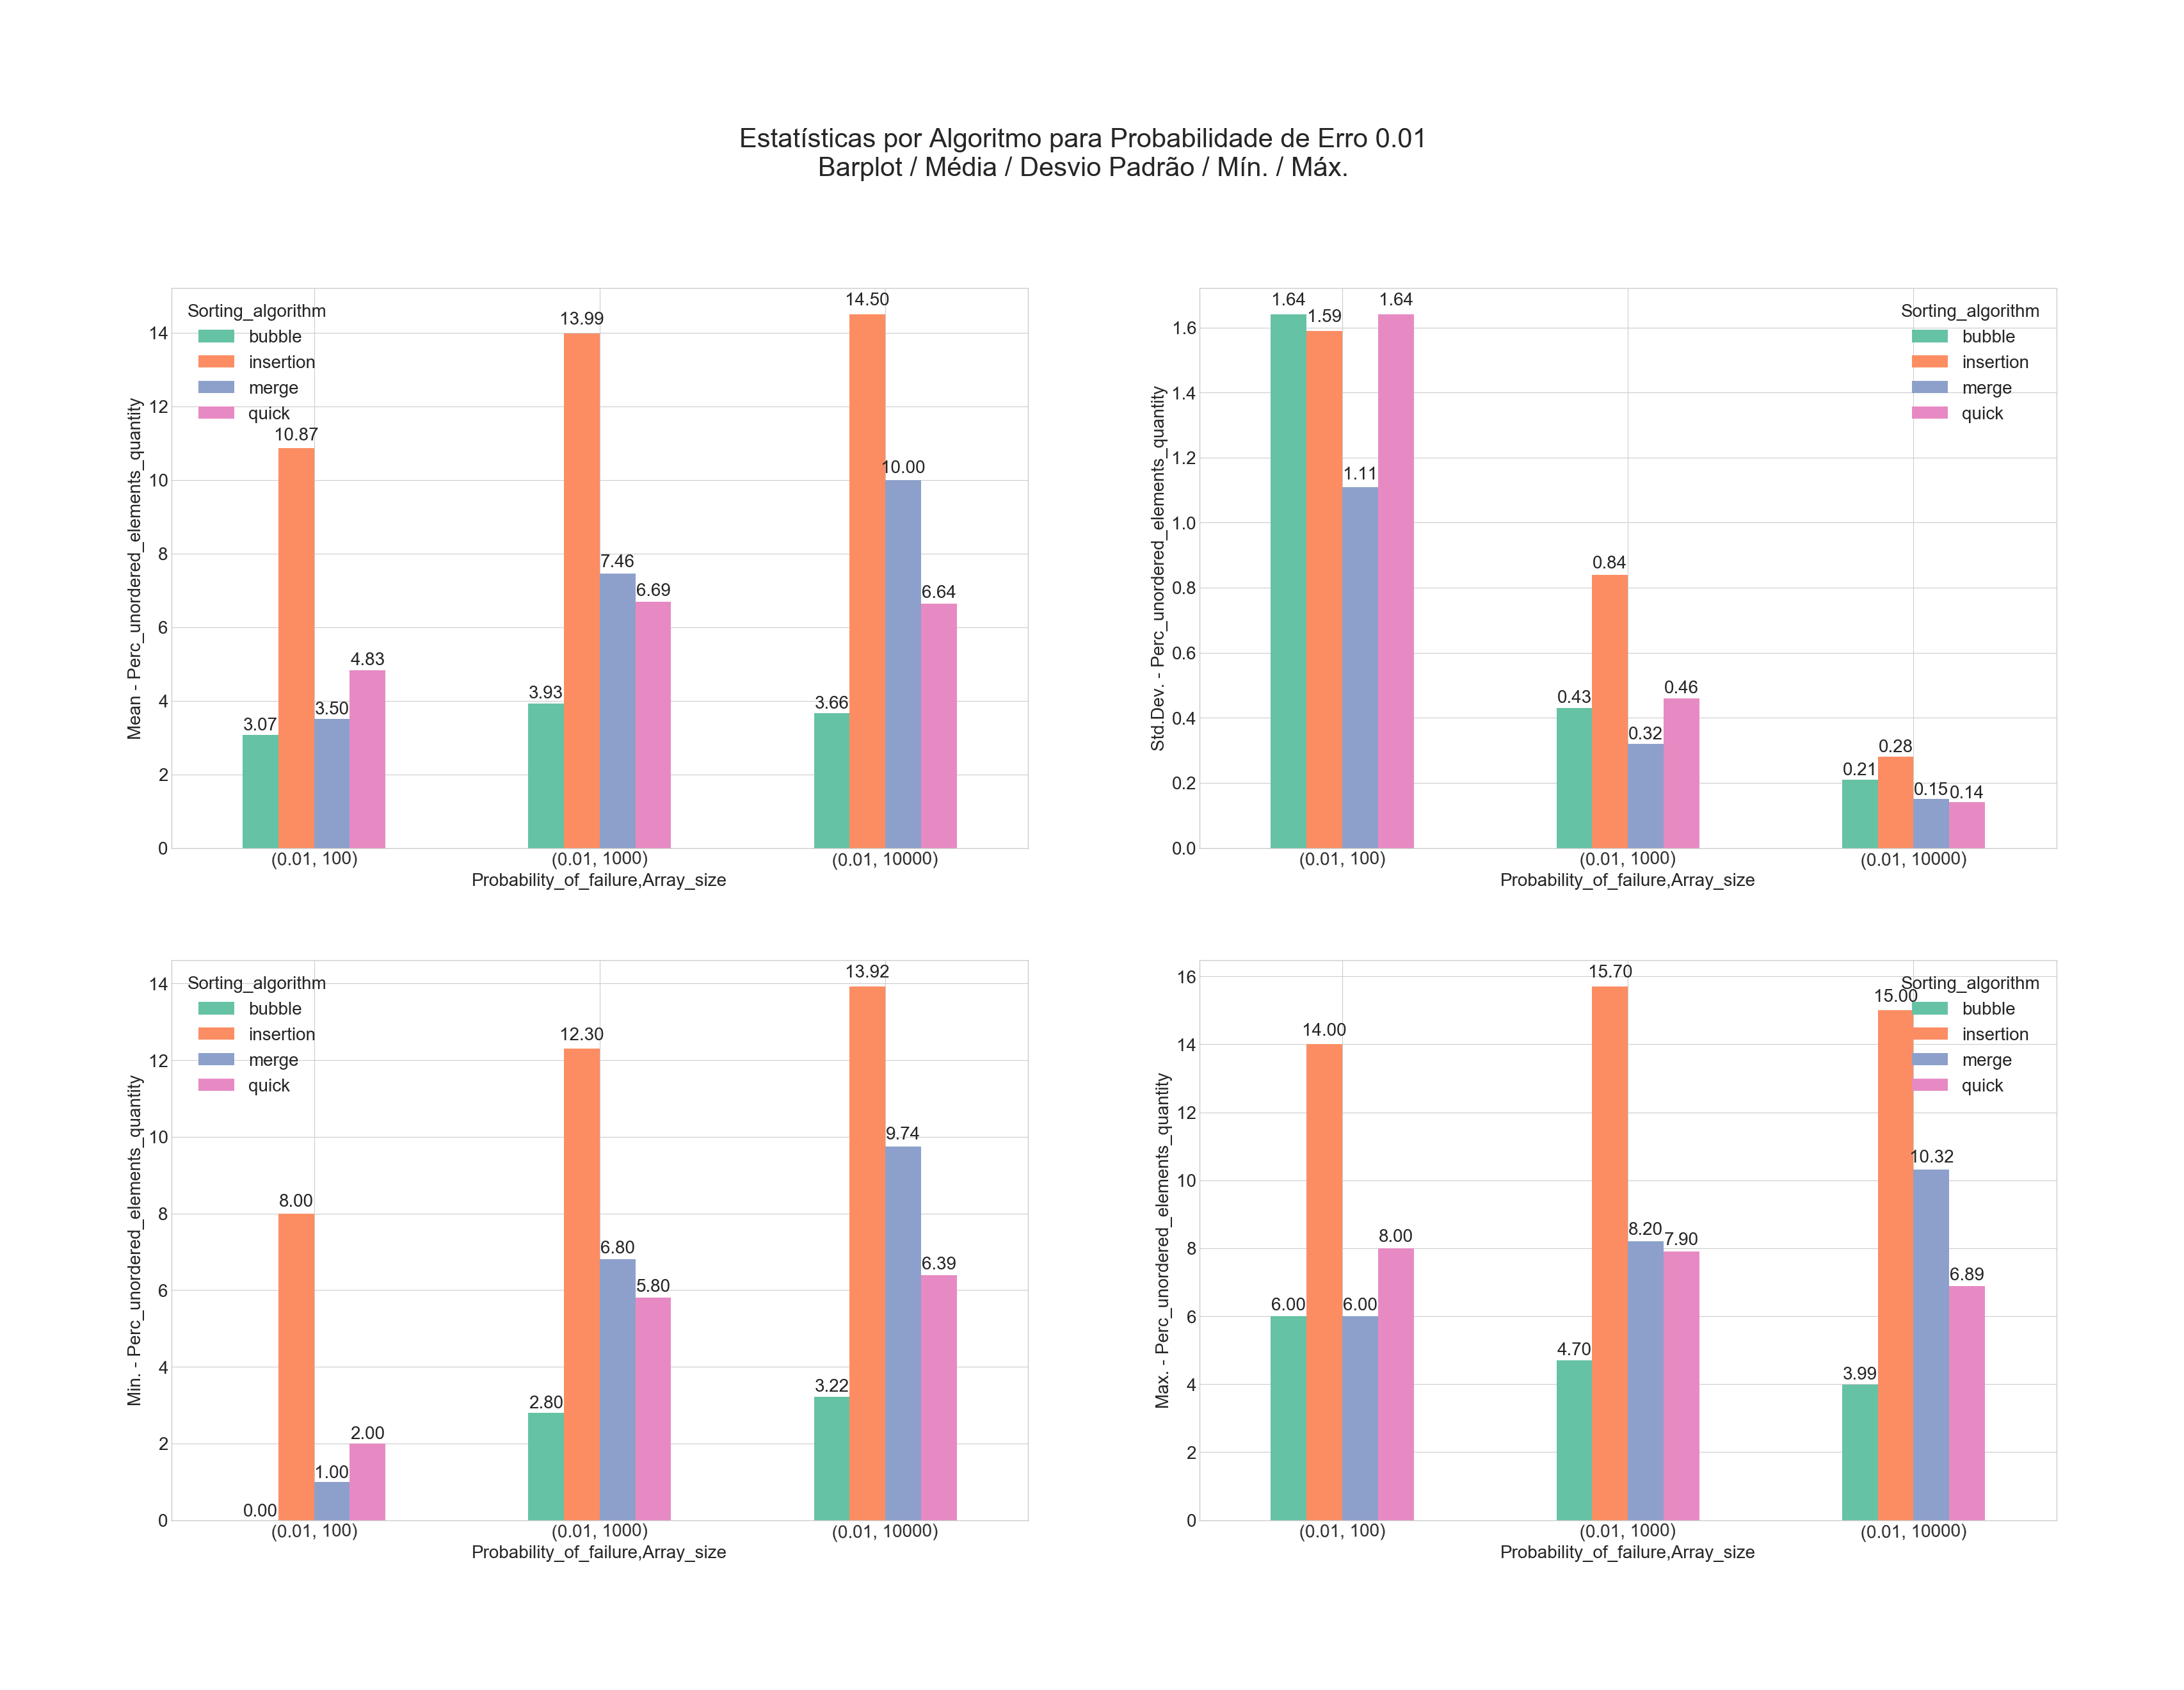
\includegraphics[scale=0.20]{figures/Estatisticas_por_Algoritmo_Prob_001.png}}
    \caption{Distribution data with \textit{probability of failure} of 0.01, all algorithms and \textit{array sizes}.}
    \label{fig-distribution-all-algorithms-001-all-sizes}
\end{figure}

\subsection{Dependente Variables Normality}

An essential step to continue the analysis is to verify if dependent variables have a normal distribution. In this work, we produced the Q-Q plot to analyze the normality visually. We also ran the Shapiro-Wilk \cite{shapiro1965analysis} test to confirm if they follow a normal distribution or not.

After the Shapiro-Wilk test, we determine that only the dependent variable \%UEQ (\textit{percentage of unordered elements quantity}) has a normal distribution related to mean for all algorithms. This situation occurs considering all possible combinations between independent variables: \textit{sorting algorithm}, \textit{probability of failure} and \textit{array size}.

Based on these results, we choose to test just the hypothesis associated with the dependent variable \%UEQ. We make use of the ANOVA method to test the hypothesis, and this method is premised the normal distribution of variables values.

Tables \ref{table-shapiro-test-lss} and \ref{table-shapiro-test-ueq} shows examples of results we get running Shapiro-Wilk test. The independent variables assume these values: \textit{probability of failure} of 0.01 and \textit{array size} of 100. The bold \textit{p-values} confirms that the data is normally distributed.

\begin{table}[H]
    \parbox{.45\linewidth}{
        \caption{Shapiro-Wilk test for \%LSS with \textit{probability of failure} of 1\% and \textit{array size} of 100.}
        \begin{center}
        \begin{tabular}{|c|c|c|}
        \hline
        \textbf{Algorithm} & \textbf{W} & \textbf{p-value} \\
        \hline
        Bubblesort & 0.854840 & 0.0007 \\
        \hline
        Insertion Sort & 0.961790 & \textbf{0.3439} \\
        \hline
        Mergesort & 0.937173 & \textbf{0.0763} \\
        \hline
        Quicksort & 0.869708 & 0.0016 \\
        \hline
        \end{tabular}
        \label{table-shapiro-test-lss}
        \end{center}
    }
    \hfill
    \parbox{.45\linewidth}{
        \caption{Shapiro-Wilk test for \%UEQ with \textit{probability of failure} of 1\% and \textit{array size} of 100.}
        \begin{center}
        \begin{tabular}{|c|c|c|}
        \hline
        \textbf{Algorithm} & \textbf{W} & \textbf{p-value} \\
        \hline
        Bubblesort & 0.934980 & \textbf{0.0666} \\
        \hline
        Insertion Sort & 0.949881 & \textbf{0.1678} \\
        \hline
        Mergesort & 0.936667 & \textbf{0.0739} \\
        \hline
        Quicksort & 0.936049 & \textbf{0.0712} \\
        \hline
        \end{tabular}
        \label{table-shapiro-test-ueq}
        \end{center}
    }
\end{table}

Q-Q plot shows that how much more blue points close to the red line, most normal is the distribution. Figure \ref{fig-qqplot-lss-001-100} below presents this graph for the dependent variable \textit{percentage of the largest subarray size} considering a \textit{probability of failure} of 1\% and a \textit{array size} of 100 for all sorting algorithms. 

\begin{figure}[H]
    \centering
    \frame{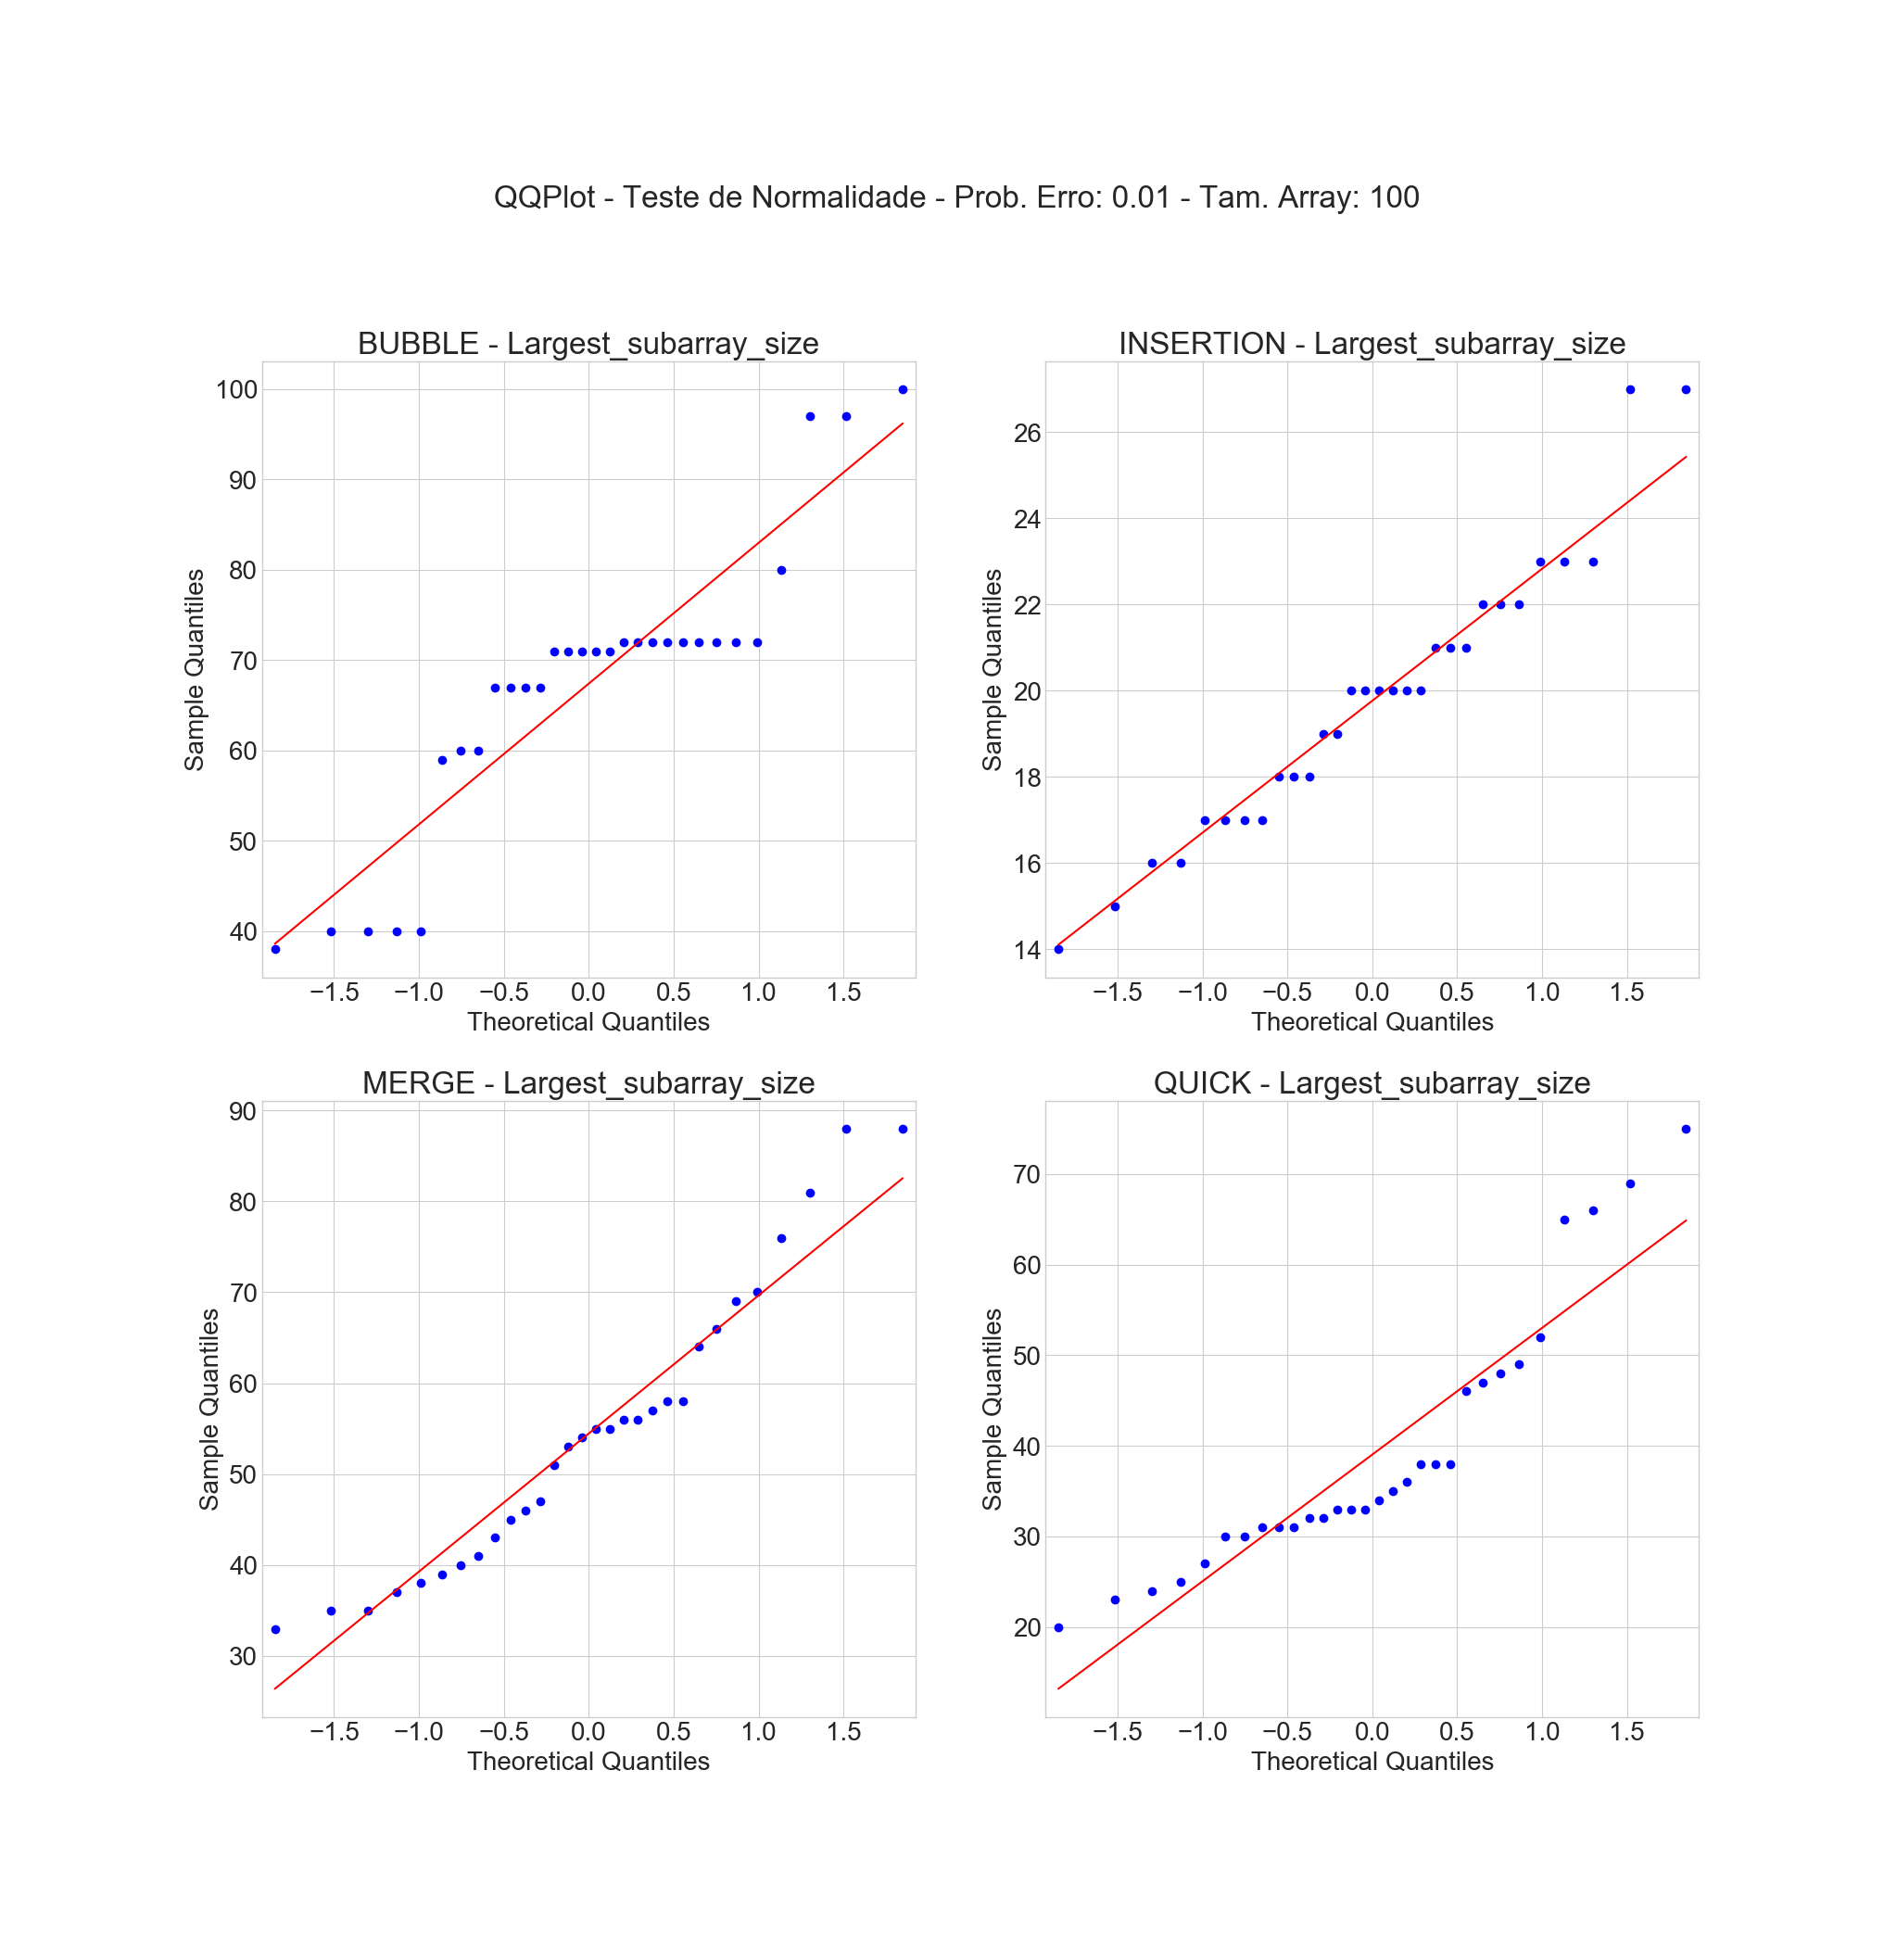
\includegraphics[scale=0.30]{figures/anova_prob_0_01_tam_100_Largest_subarray_size.png}}
    \textsf{\caption[Q-Q plot for \%LSS with \textit{probability of failure} of 1\% and \textit{array size} of 100.]{Q-Q plot for \%LSS with \textit{probability of failure} of 1\% and \textit{array size} of 100.\label{fig-qqplot-lss-001-100}}}
 \end{figure}

 Figure \ref{fig-qqplot-ueq-001-100} shows the same graph for the dependent variable \textit{percentage of unordered elements quantity} considering same values for independent variables.

\begin{figure}[H]
    \centering
    \frame{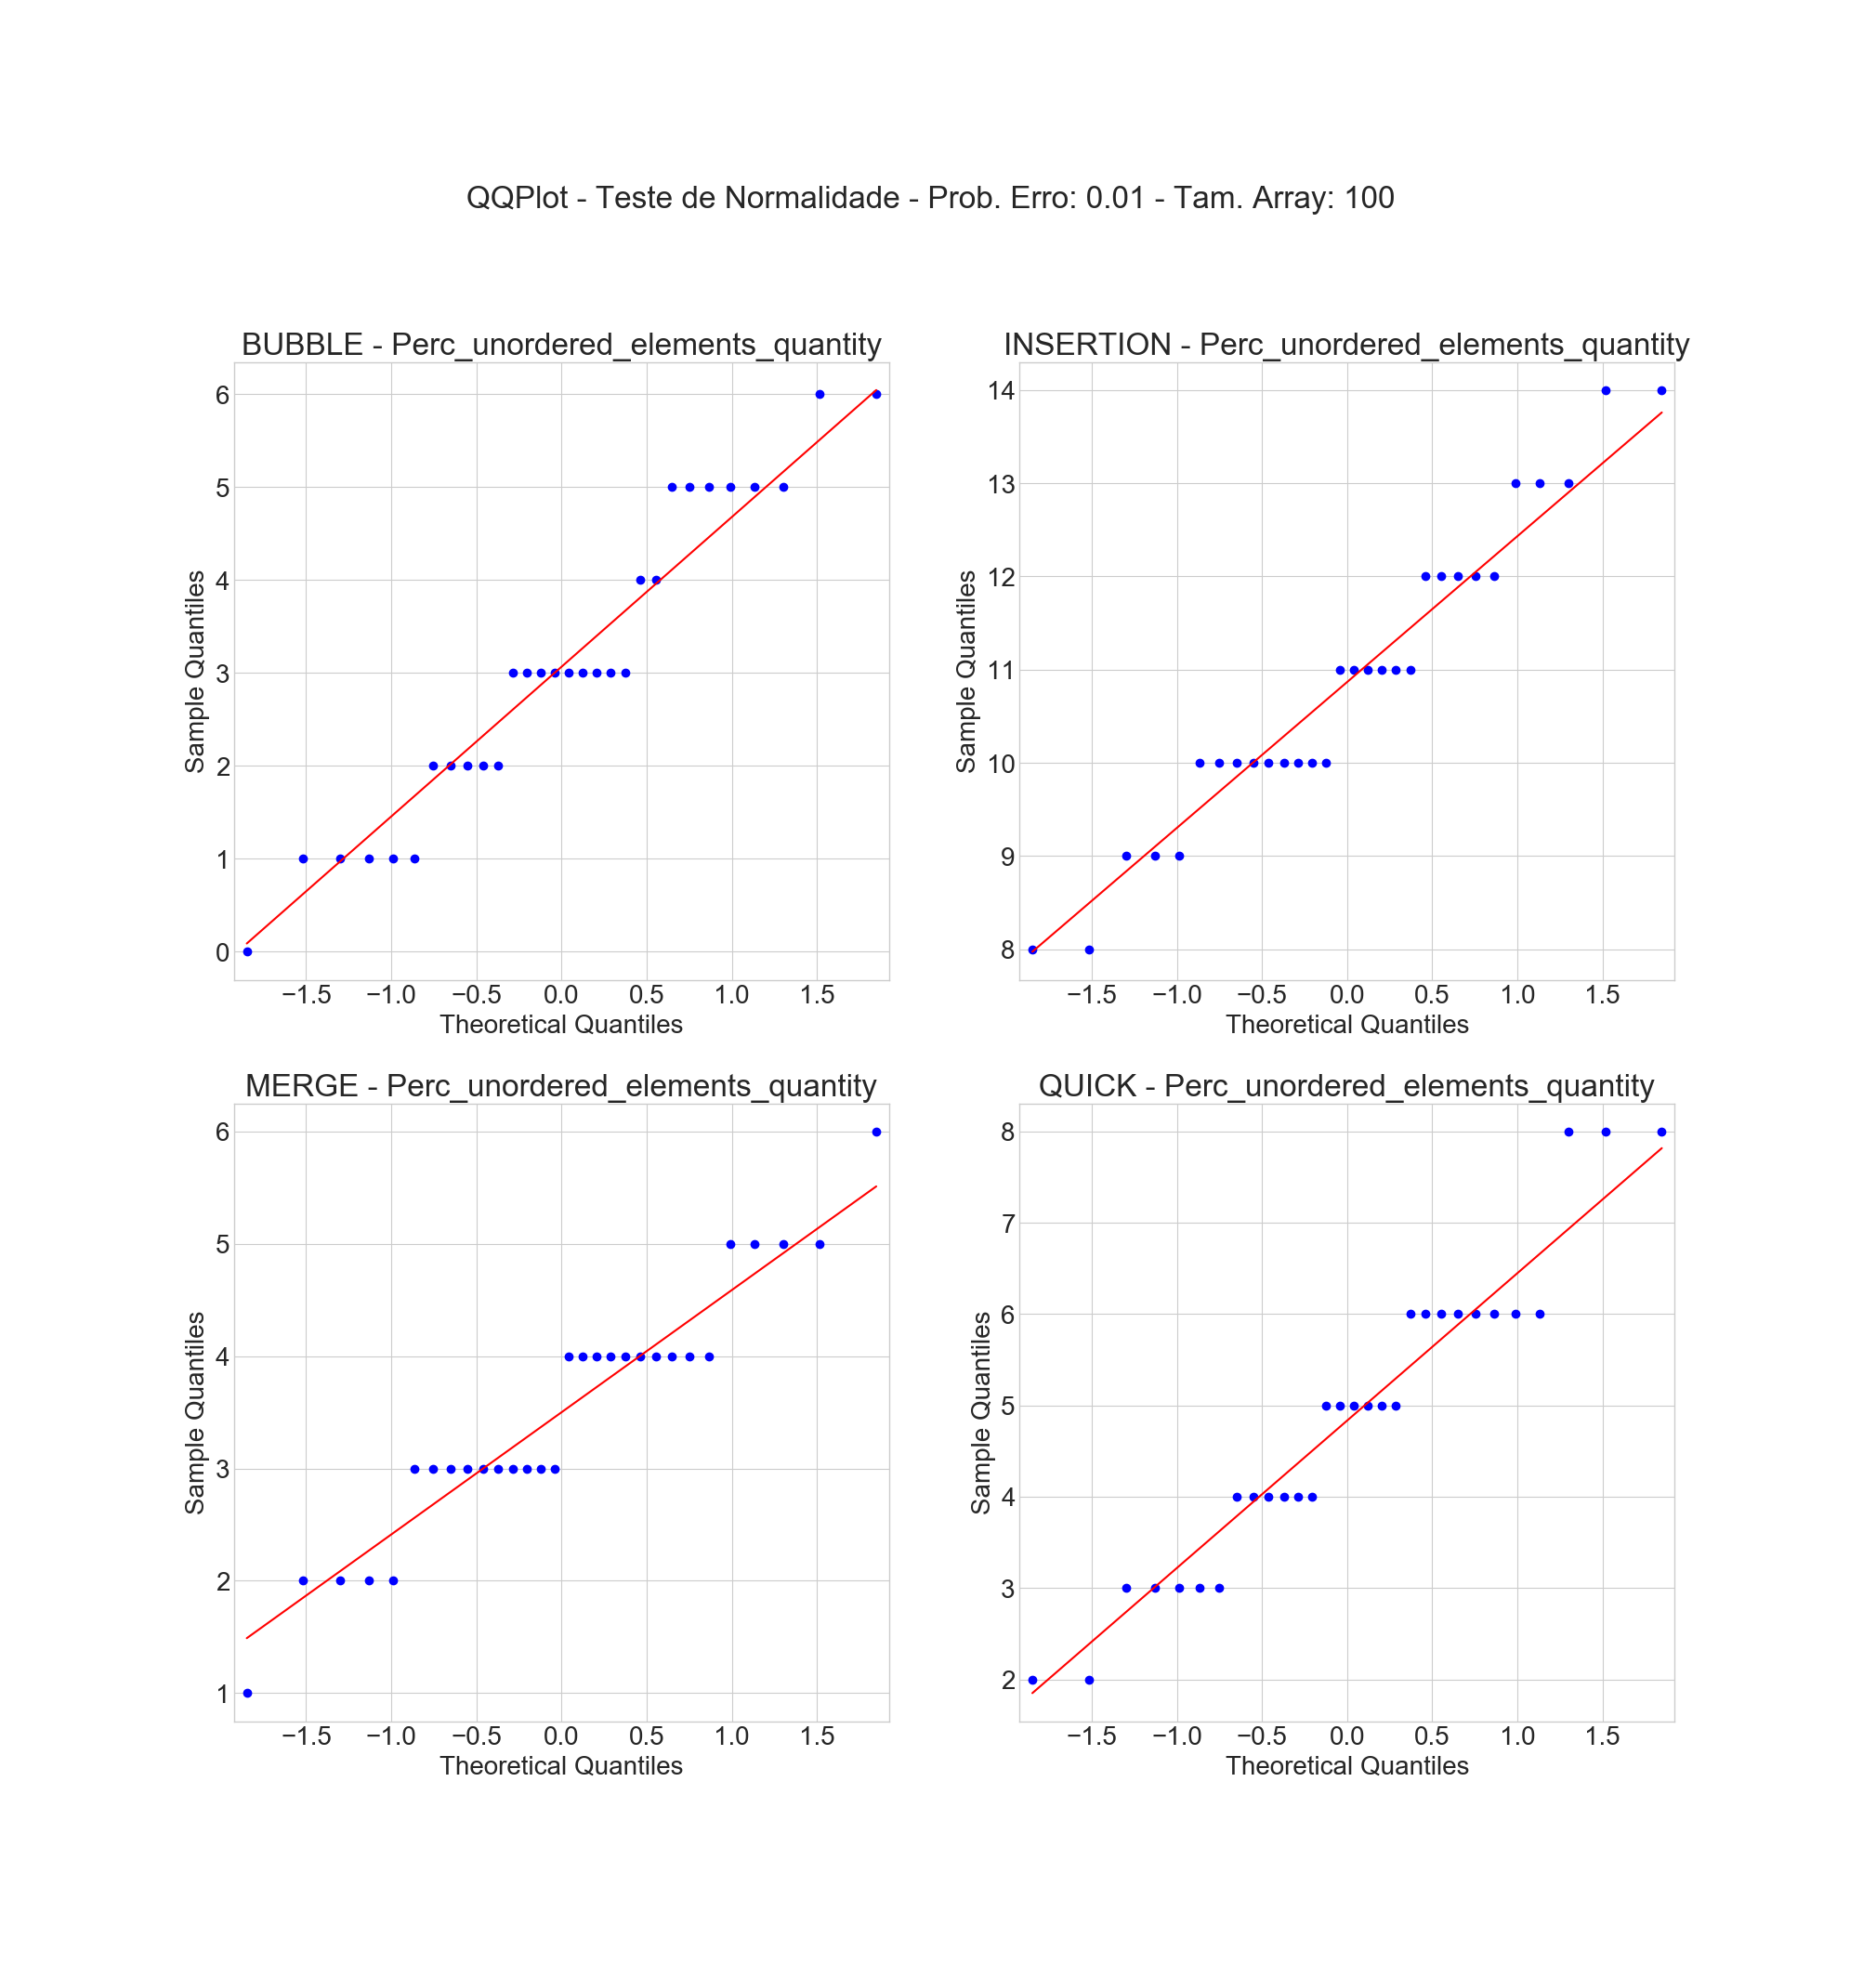
\includegraphics[scale=0.30]{figures/anova_prob_0_01_tam_100_Perc_unordered_elements_quantity.png}}
    \textsf{\caption[Q-Q plot for \%UEQ with \textit{probability of failure} of 1\% and \textit{array size} of 100.]{Q-Q plot for \%UEQ with \textit{probability of failure} of 1\% and \textit{array size} of 100.\label{fig-qqplot-ueq-001-100}}}
\end{figure}